\cotefile{74}
\scanpage{106}
\figure{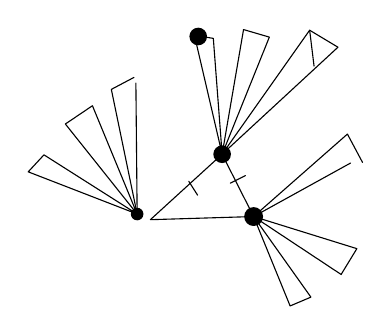
\begin{tikzpicture}[x=0.008cm,y=-0.008cm,line cap=round,line join=round]
\draw (237,514)--(351,410)--(401,509)--cycle;
\draw (216,505)--(43,438)--(68,411)--cycle;
\draw (216,505)--(102,362)--(145,333)--cycle;
\draw (216,505)--(175,307)--(211,288);
\draw (216,505)--(214,297);
\draw (351,410)--(307,221)--(337,226)--cycle;
\draw (351,410)--(385,212)--(426,224)--cycle;
\draw (351,410)--(490,213)--(535,240)--cycle;
\draw (490,213)--(497,270);
\draw (401,509)--(550,378)--(574,423);
\draw (401,509)--(555,424);
\draw (401,509)--(565,560)--(540,601)--cycle;
\draw (401,509)--(492,637)--(459,651)--cycle;
\draw (298,453)--(312,475);
\draw (364,456)--(388,444);
\fill (216,505) circle[radius=10];
\fill (351,410) circle[radius=14];
\fill (401,509) circle[radius=15];
\fill (313,223) circle[radius=14];

\end{tikzpicture}}

$\sigma_{t_0}$

\figure{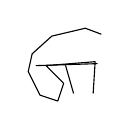
\begin{tikzpicture}[x=0.025cm,y=-0.025cm,line cap=round,line join=round]
\draw (39,4)--(31,1)--(14,5)--(4,14)--(2,23)--(8,35)--(17,38)--(20,29)--(11,20)--(36,18)--(35,34);
\draw (6,20)--(37,19);
\draw (21,20)--(25,34);


\end{tikzpicture}}

\figure{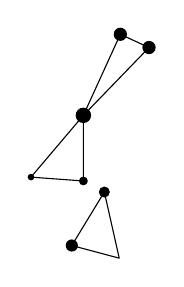
\begin{tikzpicture}[x=0.007cm,y=-0.007cm,line cap=round,line join=round]
\draw (1123,378)--(1218,266)--(1218,385)--cycle;
\draw (1218,266)--(1285,119)--(1337,143)--cycle;
\draw (1197,502)--(1256,405)--(1283,525)--cycle;
\fill (1218,266) circle[radius=14];
\fill (1285,119) circle[radius=12];
\fill (1337,143) circle[radius=12];
\fill (1123,378) circle[radius=6];
\fill (1218,385) circle[radius=8];
\fill (1197,502) circle[radius=11];
\fill (1256,405) circle[radius=10];

\end{tikzpicture}}

\figure{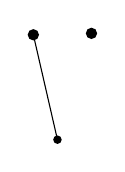
\begin{tikzpicture}[x=0.009cm,y=-0.009cm,line cap=round,line join=round]
\draw (209,699)--(243,847);
\fill (209,699) circle[radius=8];
\fill (243,847) circle[radius=6];
\fill (291,697) circle[radius=8];

\end{tikzpicture}}

\textcircled{\unsure{bons|bon}} \uline{\unsure{compl.} : $0$ \unsure{branches|boucles}} \quad a)

\figure{
\begin{tikzpicture}[x=0.035cm,y=-0.035cm,line cap=round,line join=round]

\fill (0,8) circle[radius=8];
\fill (31,5) circle[radius=5];
\fill (56,0) circle[radius=4];

\end{tikzpicture}}

par un sommet passe $0$ triangle (\deleted{\illegible{1}} : $0$ arêtes)

\noindent\rule{.69\linewidth}{.4pt}

\textcircled{\uline{\unsure{bons|bon}}} \quad $n=1$ branche \quad b)

\figure{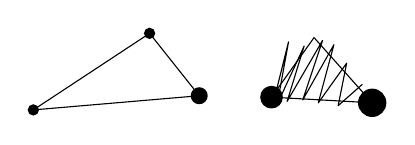
\begin{tikzpicture}[x=0.018cm,y=-0.018cm,line cap=round,line join=round]
\draw (0,54)--(82,0)--(117,44)--cycle;
\draw (168,45)--(198,3)--(239,49)--cycle;
\draw (170,46)--(180,6)--(172,50)--(191,9)--(179,48)--(204,5)--(190,47)--(212,8)--(201,49)--(221,21)--(215,51)--(232,36);
\fill (0,54) circle[radius=4];
\fill (82,0) circle[radius=4];
\fill (117,44) circle[radius=6];
\fill (168,45) circle[radius=8];
\fill (239,49) circle[radius=10];

\end{tikzpicture}}

par un sommet passe $1$ triangle exact\textsuperscript{t} (ou $2$ arêtes exact\textsuperscript{t})

\noindent\rule{.81\linewidth}{.4pt}

% slanted
\margin{cas où existe un centre (un pt auquel tt autre pt est lié) -- (unique sauf pour le cas où $S$ est \unsure{bon|borné} $=$ un triangle)}

\uline{non bons} \qquad c)

\figure{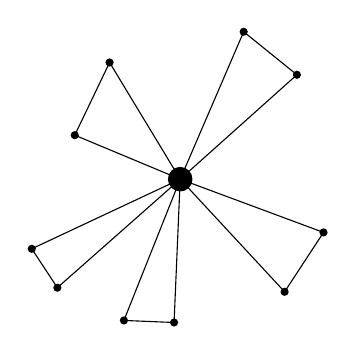
\begin{tikzpicture}[x=0.013cm,y=-0.013cm,line cap=round,line join=round]
\draw (1020,1032)--(917,989)--(951,918)--cycle;
\draw (1020,1032)--(1082,888)--(1134,930)--cycle;
\draw (1020,1032)--(1160,1084)--(1122,1142)--cycle;
\draw (1020,1032)--(1014,1172)--(965,1170)--cycle;
\draw (1020,1032)--(900,1138)--(875,1100)--cycle;
\fill (1020,1032) circle[radius=12];
\fill (917,989) circle[radius=4];
\fill (951,918) circle[radius=4];
\fill (1082,888) circle[radius=4];
\fill (1134,930) circle[radius=4];
\fill (1160,1084) circle[radius=4];
\fill (1122,1142) circle[radius=4];
\fill (1014,1172) circle[radius=4];
\fill (965,1170) circle[radius=4];
\fill (900,1138) circle[radius=4];
\fill (875,1100) circle[radius=4];

\end{tikzpicture}}

\[ n\geq 2\ \text{branches} \]

\deleted{\unsure{type}} étoile de triangles \deleted{\unsure{telle que}} \deleted{\unsure{en des sommets|à deux sommets}} tous les sommets sauf $1$ sont d'ordre $2$, \deleted{l'autre} (l'\unsure{exceptionnel|exceptionn\textsuperscript{el}} est d'ordre $\geq4$)

par tous les sommets sauf $1$ passe exact\textsuperscript{t} un triangle, pour l'excep. il y en a \deleted{\unsure{au}} au moins deux [\deleted{\unsure{et}} \unsure{i.e.|i.e} il y a au moins $4$ de sommets par lesquels passe \deleted{\unsure{un}} exact\textsuperscript{t} $1$ triangle ..]

\noindent\rule{\linewidth}{.4pt}

\uline{bons}, Par tt sommet passe au moins $\unsure{3|2}$ triangles

% archive sheet number: 105
